\chapter{降压所整定计算}
本章以降压站为例分析各级保护的整定配合,该站的基本参数如下(\ref{降压所}):\par 
10kV电力变压的容量为315kVA,短路阻抗为4.01\%,变压器最大负荷电流为18.2A,高压侧电流互感器变比为50:1。

\begin{figure}[h] %H为当前位置,!htb为忽略美学标准,htbp为浮动图形
	\centering %图片居中
	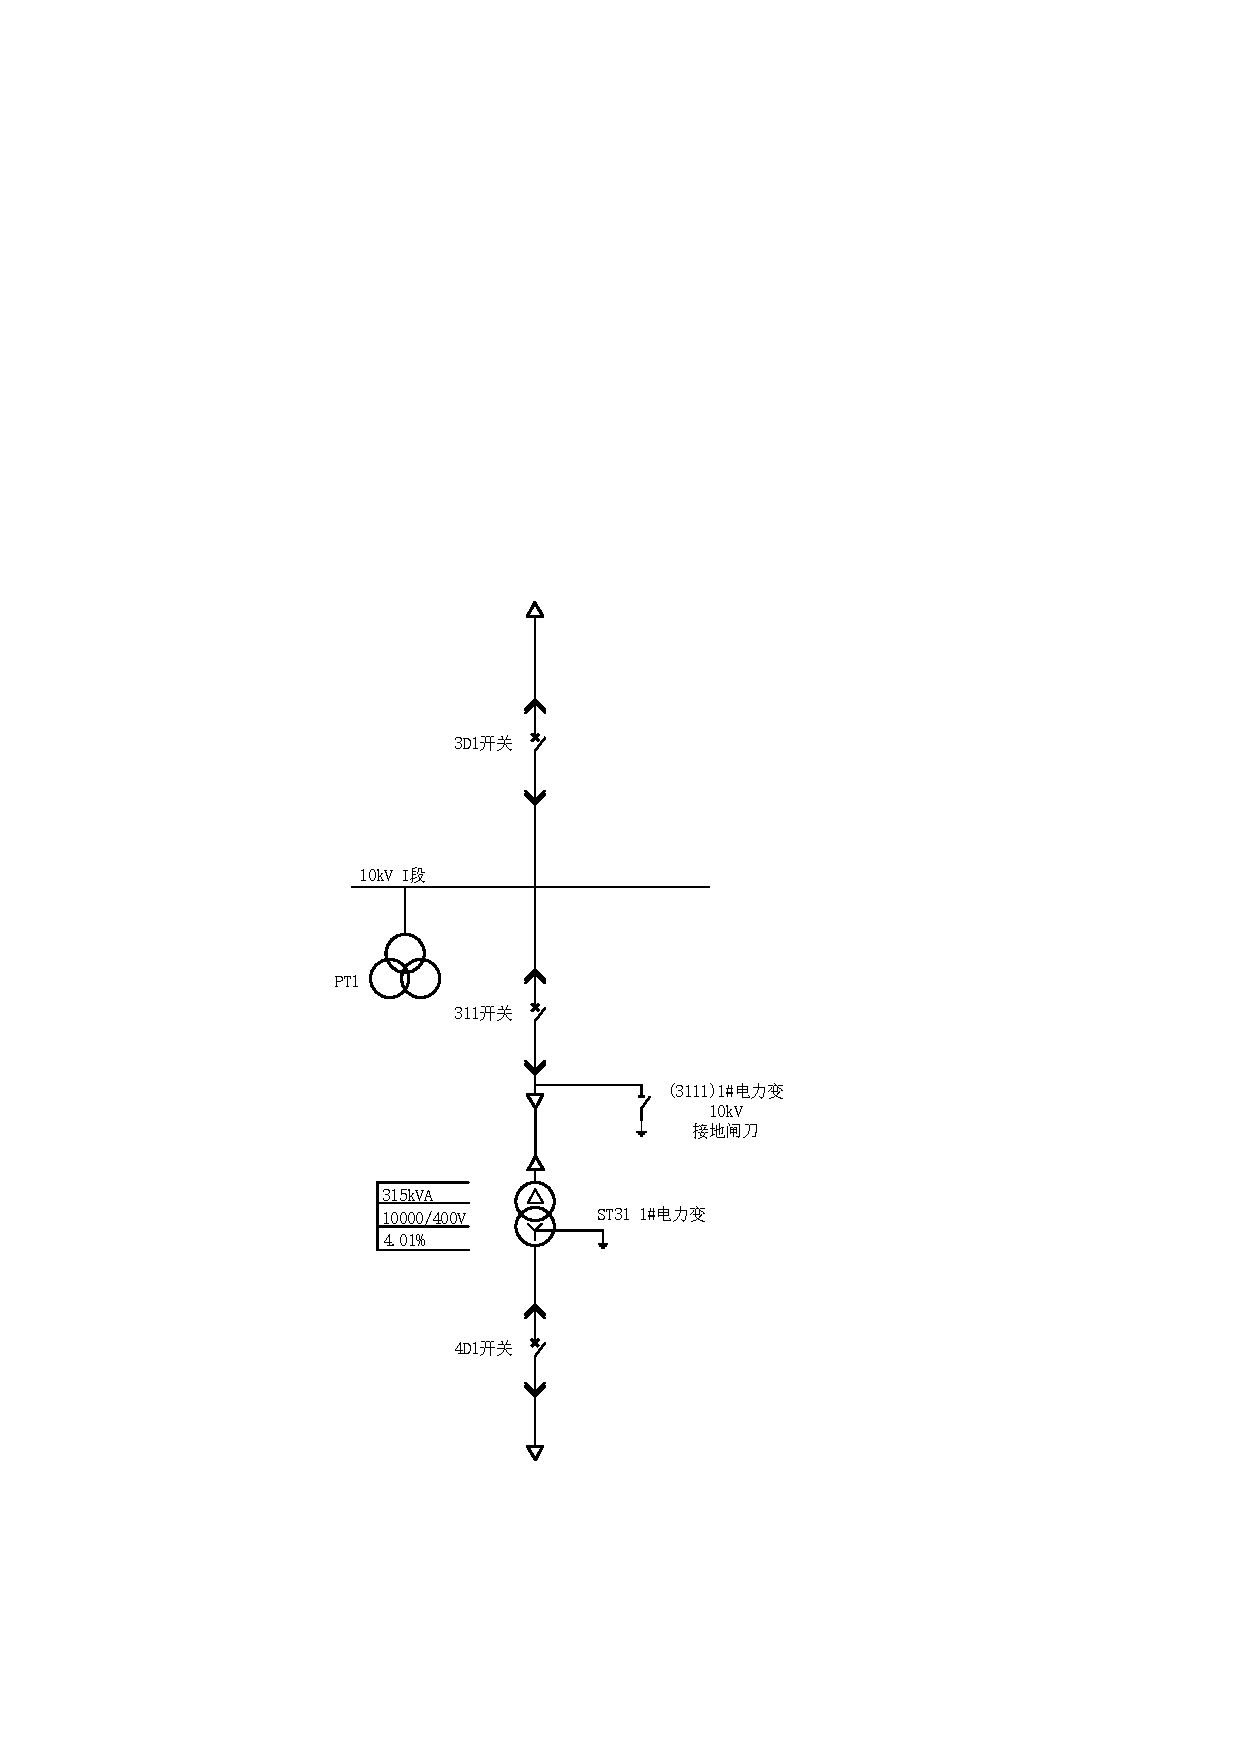
\includegraphics[width=0.5\textwidth]{降压所.pdf} %插入图片,[]中设置图片大小,{}中是图片文件名
	\caption{降压所} %最终文档中希望显示的图片标题
	\label{降压所} %用于文内引用的标签
\end{figure}
\section{电力变压器开关整定值计算}
选取基准容量$S_{b}=100MVA$,则各基准电压及电流分别为:\par 
高压侧:$U_{bI}=10kV$则$I_{bI}=\frac{S_b}{\sqrt{3}U_{bI}}=\frac{100}{\sqrt{3}\times 10.5}=5.5kA$\par 
低压侧:$U_{bII}=0.4kV$则$I_{bII}=\frac{S_b}{\sqrt{3}U_{bII}}=\frac{100}{\sqrt{3}\times 0.4}=114.3kA$\par  
变压器电抗标幺值:$X_{*k}=\frac{X_T\%}{100}\times \frac{S_b}{S_{T1}}=\frac{4.01}{100}\times \frac{100}{0.315}=12.73$
$$X_{*\sum{}}=12.73$$\par 
短路电流标幺值为:$I_{*k}=\frac{1}{12.73}=0.0786$\par 
在低压侧发生三相短路时实际短路电流为:$$ I^{\left( 3 \right)}=I_{*k}\times I_{bII}=0.0786\times 144.3kA=11342A $$
\subsection{311开关保护装置装置速断保护($I>>$)整定计算}
$$
I>>=K_{rel}\cdot \frac{I^{\left( 3 \right)}}{n_T}=1.25\times \frac{11342}{25}\div 50=11.34
$$
整定值:取$I>>=11.4(A)$\newline 
时间:0.035s。
\subsection{311开关保护装置过电流保护(I>)整定计算:}
过电流保护按躲过变压器的最大负荷电流为18.2A为原则,取可靠系数$K_{rel}=1.5$,过负荷系数$K_{gh}=2$,于是有:
$$
I>=K_{rel}\cdot \frac{K_{gh}I_{TN}}{n_T}=1.5\times 2\times 18.2\div 50=1.092\left( A \right) 
$$
整定值:取$I>=1.1(A)$\newline 
时间:0.4s。\par 
按变压器低压侧发生两相短路时的短路电流来校验灵敏度$K_{sen}$,于是有:
$$
K_{sen}=\frac{0.866\times 11342}{25\times 1.1\times 50}=7.14>2  \text{满足要求}
$$
\subsection{311开关保护装置反时限过电流保护整定计算:}
计算过程如下:
$$
I_{set}=K_{rel}\cdot \frac{I_{TN}}{n_T}=1.25\times 18.2\div 50=0.455\left( A \right) 
$$
取$T_{p}=0.4$
$$
t=\frac{0.14}{\left( \frac{I}{I_{act}} \right) ^{0.02}-1}\cdot T_p=\frac{0.14}{\left( \frac{{I}}{0.455} \right) ^{0.02}-1}\times 0.4
$$
当变压器过负荷50\%运行时,$I=\left( 1+50\% \right) \times \frac{I_{TN}}{n_T}=1.50\times 18.2\div 50=0.546\left( A \right) $\par 
此时的动作时限为:$$
t=\frac{0.14}{\left( \frac{I}{I_{act}} \right) ^{0.02}-1}\times T_p=\frac{0.14}{\left( \frac{0.546}{0.455} \right) ^{0.02}-1}\times 0.4=15.33s
$$
即当变压器过负荷50\%时,反时限保护将启动,并在延时$15.3s$后发出报警或者跳闸信号。
\section{与上游$10kV$断路器整定配合}
根据降压站10$kV$环网最大负荷电流说明,$10kV$进线开关的最大负荷电流为$50A$,而该开关的定时限过电流定值为$I>80A,t>0.3s$。因此,该开关保护整定值的裕度为$80/50=1.6$,故该开关可以可靠躲过系统最大负荷电流。当其作为电力变311开关后背保护时,其灵敏度为$$t=\frac{0.14}{\left( \frac{I}{I_{act}} \right) ^{0.02}-1}\times T_p=\frac{0.14}{\left( \frac{0.546}{0.455} \right) ^{0.02}-1}\times 0.4=15.33s
$$,因此,在311保护失灵时,301作为后备保护能够可靠动作,切除故障。\par 
在时限的配合上,301过电流保护动作时限设定为0.3s,而311保护的速断时限设定为0.03s。因此,在短路故障的情况下,301和311保护均起动,但311保护保护先动作切除故障点后,301保护自动复归,从而保证保护的选择性。
\section{与下游400$kV$断路器整定值配合}
除了与10$kV$进线配合外,311开关保护的过电流定值还需要与下游400V断路器401开关保护定值相配合,在计算时按躲过后端最大负荷电流为原则,且取一定的裕度。在实际运用中,401开关保护的长时限整定值为600A,归算到10$kV$一次侧电流为24A。因此,此时311过电流保护整定值的裕度为$55/24=2.3>2$,能可靠躲过最大负荷电流,保护可靠不动作。\par 
当作为401开关的后备保护时,应该具有足够的灵敏度。401开关短路电流设置为$8\times600=4800A$,动作时限为0.1s,归算到$10kV$侧311处的稳定电流为4800/25=192A。因此,在401后端发生短路的情况下,作为401开关的后备保护,其灵敏度为$K_{sen}=192/55=3.49>2$,能满足使用要求。如图\ref{降压所}所示。
\addtocounter{page}{-1}